\documentclass[11pt]{article}   	% use "amsart" instead of "article" for AMSLaTeX format
\usepackage[margin=1in]{geometry}
\usepackage{textcomp}
\usepackage{geometry}                		% See geometry.pdf to learn the layout options. There are lots.
\geometry{letterpaper}                   		% ... or a4paper or a5paper or ...
%\geometry{landscape}                		% Activate for rotated page geometry
%\usepackage[parfill]{parskip}    		% Activate to begin paragraphs with an empty line rather than an indent
\usepackage{graphicx}				% Use pdf, png, jpg, or eps§ with pdflatex; use eps in DVI mode
\usepackage{caption}
\usepackage{subcaption}								% TeX will automatically convert eps --> pdf in pdflatex
\usepackage{color}
\usepackage{amssymb}
\usepackage{amsthm}
\usepackage{url}
\newtheorem{theorem}{Theorem}
\newtheorem{definition}{Definition}
\usepackage{natbib}
\usepackage{xcolor}
% removed hyperref because of arXiv complaining
\usepackage{float}
\usepackage{rotating}
\usepackage{adjustbox}
\usepackage[font=small,labelfont=bf]{caption}
%\usepackage{changes}
\usepackage{changes}
\usepackage[colorlinks=false]{hyperref}
\usepackage{wrapfig}
\definechangesauthor[name={George Chacko}, color=blue]{gc}

\usepackage{authblk}
\title{Well-Connected Communities in Real-World Networks}
\author[1]{Minhyuk Park\thanks{Minhyuk Park and Yasamin Tabatabaee contributed equally}}
\author[1]{Yasamin Tabatabaee}
\author[1]{Baqiao Liu}
\author[1]{Vidya Kamath Pailodi\thanks{Vidya Kamath Pailodi and Vikram Ramavarapu contributed equally}}
\author[1]{Vikram Ramavarapu}
\author[1]{Rajiv Ramachandran}
\author[2]{Dmitriy Korobskiy}
\author[3]{Fabio Ayres}
\author[1,4]{George Chacko\thanks{chackoge@illinois.edu}}
\author[1]{Tandy Warnow\thanks{warnow@illinois.edu}}
\affil[1]{Department of Computer Science, University of Illinois Urbana-Champaign, Urbana, IL 61801, USA}
\affil[2]{NTT DATA, McLean, VA 22102, USA}
\affil[3]{Insper Institute, S\={a}o Paulo, Brazil}
\affil[4]{Office of Research, Grainger College of Engineering, University of Illinois Urbana-Champaign, Urbana, IL 61801, USA}

% \setlength{\parindent}{0pt}
%SetFonts

% ORCID IDs

% Baqiao Liu: 0000-0002-4210-8269
% Tandy Warnow: 0000-0001-7717-3514
% George Chacko: 0000-0002-2127-1892

\begin{document}
\maketitle

\abstract{Community detection in real-world networks is typically addressed through the use of graph clustering methods that partition the nodes of a
network into disjoint subsets. While  the definition of community may vary, it is generally accepted that elements of a community should be ``well-connected".
Applying a mild definition of well-connectedness, we explore features of clusters generated by the Leiden algorithm  and the Iterative K-core clustering algorithm. We evaluate
clusters produced  by these two approaches for their susceptibility to become disconnected by the deletion of a small number of edges, and find that both methods produce some
clusters that are poorly connected  when applied to real-world networks.  We use a modular pipeline to enable well-connected output clusters that allows a user-specified criterion
for a valid community considering cluster size and minimum edge cut size. We describe the use of this pipeline on real world networks and benchmark networks.
The differences we observe between real world and the synthetic networks are compelling: clusters computed on synthetic networks  generated by the LFR methodology are more well-connected
than those clusters produced from real-world networks. Since an assumption of the LFR network generation process  is that every vertex  is in a community, the results of this study
underscore the difference between synthetic and real world networks and suggest that community structure is not globally found within real-world networks. }

\clearpage

\section{Introduction}

The problem of finding communities in complex networks can be posed as a {\em graph partitioning} problem, where the input is a network (a graph with vertices and edges) and the
objective is a partitioning of the vertices into disjoint subsets, so that each of the subsets represents a community \citep{Girvan_2002,Newman_2004}. Community
detection in  large networks has broad applications that include identifying research areas and author communities \citep{Waltman_2012,Li2014,Fiallos2017,Traag_2019,Chandrasekharan_2020,Wedell2022}.

Disjoint partition is a  common approach to community detection studies \citep{Fortunato2022,Fortunato2010} although variations on the partitioning theme arise from different scientific interests \citep{Coscia2011,Schaub2017}.
A common feature of these different formulations is that  the elements of a community are more connected to each other than to those outside the community. In other words, a community
should be {\em well-connected}.
Using graph-theoretic terminology, a cluster is said to be well-connected if it does not have a small edge cut, which means that there should not be a small set of edges whose deletion
disconnects the cluster; see discussion in \cite{Traag_2019}. A tree  (i.e., a cluster that has no cycles) is  a compelling example of a poorly connected cluster since every edge in  a tree is a cut edge (i.e.,  removal of a single edge
disconnects the cluster).

While the concept of being well-connected depends on the size of the edge cut, the definition of what is ``too small" can be formulated in two natural ways. One such  approach, which is used in
providing guarantees for the widely used Leiden algorithm \citep{Traag_2019}, specifies the minimum size of an edge cut as a function of the the split  of the cluster into two parts produced
when the edge cut is removed from a cluster. Specifically, the guarantee provided   in Equation D1 in the supplementary information in \cite{Traag_2019}) for an optimal clustering under the Constant Potts Model (CPM), which is the default optimization criterion for Leiden, is that the edge cut size be at least the resolution factor   times the number of possible edges between the two  parts. Writing this formally, and allowing $\gamma$ to be the resolution factor, then Equation D1 asserts that every edge cut $E_0$ in a Constant Potts Model (CPM)-optimal clustering is guaranteed to satisfy

 \begin{equation}
 ||E_0|| \geq \gamma ||A|| \times ||B||
 \label{eqn:cpm-bound}
 \end{equation}
where $||.||$ denotes the number of elements in the set and $E_0$ splits the cluster into two sets, $A$ and $B$.
Note that this is a {\em lower bound} on the size of an edge cut produced in an optimal CPM-clustering.
Note  that this guarantee is strongest (meaning the lower bound is largest) when $A$ and $B$ are approximately the same size, and is weakest when the
edge cut separates a single node from the remainder of the cluster. Note also that this bound depends on the size of the cluster and on   the user-specified value for $\gamma$.

As we show below, the guarantee for CPM-optimal clusters may be weak for small to moderate clusters, especially for those that are close to being stars; it will even permit relatively
large star-clusters (i.e., clusters containing a single node that is adjacent to all the remaining nodes).

\begin{figure}[h!]
\centering
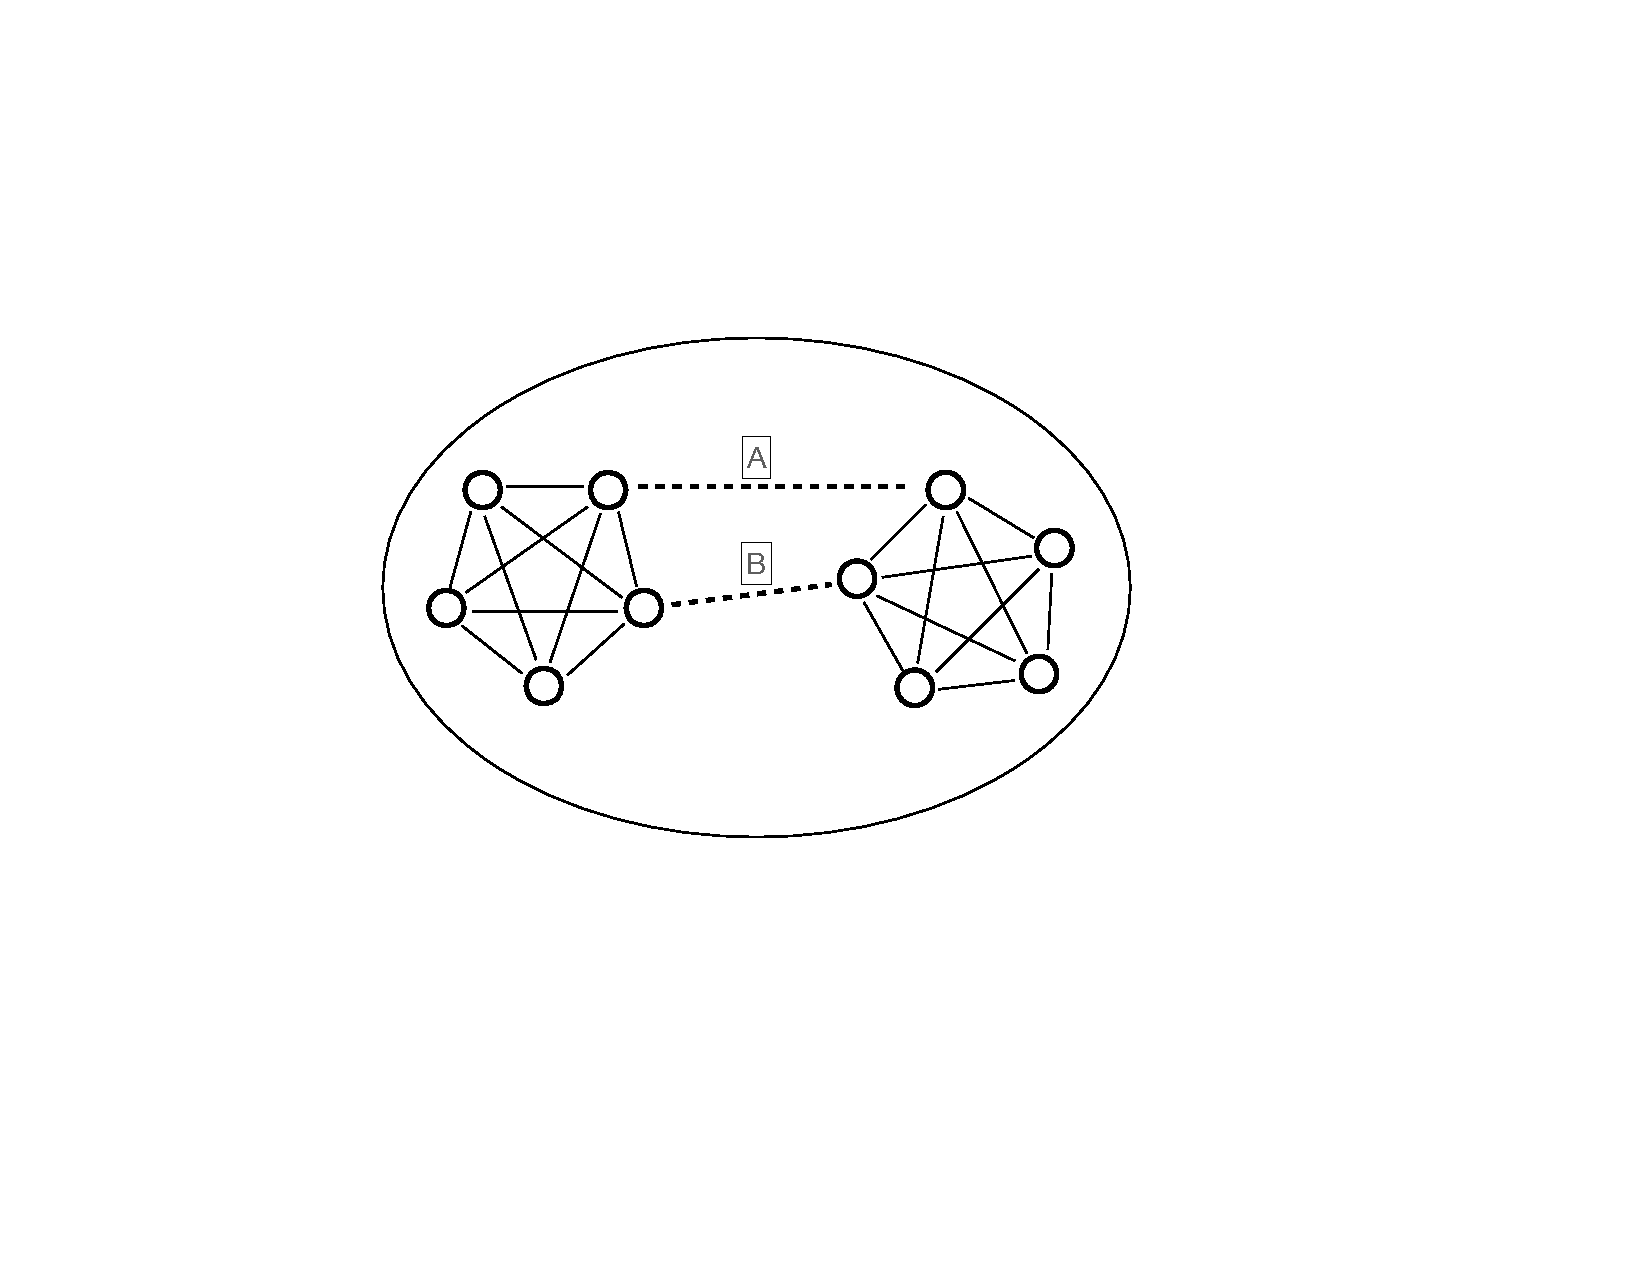
\includegraphics[width=0.5\textwidth]{figs/fig_clique.pdf}
\caption{Illustrating well-connected using Equation \ref{eqn:our-bound}. The network has two 5-cliques connected by two possible edges (dashed lines), labelled $A$ and $B$.
Each of the 5-cliques is a valid community according to Equation \ref{eqn:our-bound}, but we question whether the merger of the two 5-cliques is also valid.
According to Equation \ref{eqn:our-bound}, the minimum edge cut size  must be at least 2 for a cluster with 10 nodes to be considered well-connected.
Therefore, if only one of the edges $A$ and $B$ is present in the graph, the merged cluster  would not  be considered well-connected.
However, if both of these edges is in the network, merging the two clusters into one would produce a cluster that passes our minimum connectivity test.
On the other hand, for Equation \ref{eqn:cpm-bound}, whether the cluster formed by merging the two cliques is adequately well-connected depends on the resolution parameter, $\gamma$ (see text).}
\label{fig:2cliques}
\end{figure}

As an alternative to the bound given in Equation \ref{eqn:cpm-bound},  we consider the
following definition for well-connected.
Specifically, we require that the size of an edge cut  $E_0$  of cluster $C$ be above some function that depends only on $||C||$.
Under this definition, a cluster would be considered well-connected if every edge cut, independent of the sizes of the
two sets it creates when deleted, is large enough.
As a simple example, we consider the bound $|E_0|| > \log_{10}(||C||)$.  To enable a comparison to Equation \ref{eqn:cpm-bound}, we rewrite this  as
\begin{equation}
  ||E_0|| \geq  \lfloor \log_{10}(||C||) \rfloor +1
  \label{eqn:our-bound}
  \end{equation}
where $||.||$ denotes the number of elements in the given set and
$\lfloor . \rfloor$ is the floor (largest integer at most the size of the given value).

For example, when $||C|| \leq 9$, the bound in Equation \ref{eqn:our-bound} only enforces that the cluster be connected, when
$10 \leq ||C|| < 100$ it requires that  the cluster not have any cut edges (single edges that disconnect the cluster), etc.
This formulation offers a relatively weak bound for large clusters (i.e., when   $||C||$ is large), but does provide  a stronger constraint on small to moderate-sized clusters than the formulation based on Equation \ref{eqn:cpm-bound}.

We demonstrate this concept in Figure \ref{fig:2cliques}, where we have two cliques, each of size 5, in a network; if both the dashed edges (A and B) are present, then
merging the two cliques into a single cluster meets the minimum edge connectivity requirement (which is that the minimum edge cut must be of size at least two); however,
if only one edge is present, we cannot merge the two cliques and still have adequate edge connectivity.
On the other hand, for the CPM-based guarantee, whether the cluster formed by merging the two cliques is adequately well-connected depends on the resolution parameter, $\gamma$.
For example, if $\gamma=0.1$, then even if both edges are present, the cluster would not be considered well-connected.
If instead $\gamma=0.01$, then even if only one edge is present, the cluster would be well-connected.


Thus, the two approaches provide guarantees about clusters being well-connected for different size clusters, with the first approach (Equation \ref{eqn:cpm-bound}) being a stronger
guarantee for large clusters and the second  (Equation \ref{eqn:our-bound}) a stronger guarantee for small to moderate-sized clusters.
Understanding the differences in these guarantees is important, and is part of this study.

To explore well connectedness in community detection, we performed a study to evaluate  clusters produced by two different clustering methods:
the Leiden algorithm  \citep{Traag_2019}, and Iterative K-core Clustering (IKC) \citep{,Wedell2022}.
We designed a pipeline to work with both Leiden and IKC that would ensure that all output clusters satisfy two constraints for being valid communities: (1) each cluster meets a minimum user-specified size requirement
and (2) each cluster is well-connected according to   Equation \ref{eqn:our-bound}.
Also, (3) we ensure that each cluster is produced  by applying the selected clustering method to specified subnetworks.


The pipeline takes a Leiden or IKC clustering as input and then minimally modifies the clustering to ensure that all returned clusters meet these three requirements.
To achieve this, it  first removes all clusters that fail to meet the minimum size specified by the user; we study this method using 11 for this minimum size since we consider any cluster of size at most 10 to be
too small to be practically informative. Since any cluster that is a tree will fail our connectivity requirement when it has 10 or more vertices, we also remove all trees that remain.
After these two preprocessing steps are complete we move to the heart of the algorithm, the ``Connectivity Modifier".

Within the Connectivity Modifier, we repeatedly examine clusters to see if they are well-connected, according to our requirement.
To do this, we use the VieCut \citep{Henzinger2018,Henzinger2019}  software for finding minimum edge cuts in graphs.
If the cluster does not have a small edge cut, i.e., all its edge cuts are at least the minimum size), then the cluster is not modified by the Connectivity Modifier,
and is returned in the output.
Otherwise, the cluster is processed in a recursive fashion: first we delete the small edge cut, then we recluster the components that are created using the method specified for the input clustering
and then we recurse on each cluster that is produced. At the end of this process, every cluster that remains is well-connected, by our definition.
Moreover, every cluster that we return has been produced by Leiden, either applied to the original network or to a subnetwork created by deleting small edge cuts.
Thus, this pipeline meets properties (1) and (3), as  described above.
%\textcolor{blue}{Tandy should we put in a sentence on why we recluster?}

Note that after running the Connectivity Modifier, we have a set of clusters that are all well-connected, but some of them may be below our minimum size (default: 11).
Hence, we then check the remaining clusters to see if they are too small (at most 10 nodes), and if so we remove them.
The result of this multi-stage process is a set of clusters that meet all three required properties.
Note also that we never modify an input cluster that is sufficiently large
and meets our edge-connectivity requirement, and that every cluster that is produced is a sub-cluster of the original clustering.

Using this pipeline, we evaluate clusterings produced by Leiden and IKC for a number of different networks, including two large citation networks: the Open Citations Network with 75,025,194 vertices and 1,363,605,603 edges, and the Curated Exosome Network studied 
in \cite{Jakatdar_2022} with 75,025,194 vertices and 1,363,605,603 edges.
We find that both clusterings produce  some clusters that  fail our minimal requirements for community structure, although the extent to which these violations occur depends on the network and (in the case of Leiden) the resolution parameter. 
We also find that Leiden clusterings can reduce substantially  in node coverage (i.e., percentage of the network vertices that are found in non-singleton
clusters)  after being run through this pipeline.
These trends suggest the intriguing possibility that for some  real world networks, only a reduced subset may exhibit valid community structure,
thus calling into question the assumption that  clustering methods should place all nodes in communities. 


%In sum, the pipeline we provide enables
%the user to minimally modify a given Leiden or IKC clustering to ensure that all final clusters are well-connected, and in turn also explore the degree to which the study network exhibits
%community structure throughout the node set. The pipeline is also very flexible, allowing the user to modify the requirements for validity in output clusters (i.e., changing the minimum cluster
%size and/or modifying the function for the size requirement for an edge cut).

\section{Materials and Methods}

\subsection{Notation and definitions}
We begin with basic notation and definitions.
\begin{itemize}
\item We assume that all networks have no self-loops and no parallel edges.
\item A cluster $C$ is a subset of the vertices in the network. The number of vertices in $C$ is denoted by $||C||$.
\item A tree cluster is a cluster that has no cycles.
\item A clustering is a partitioning of the input network vertices into disjoint sets.  Singleton clusters are typically
discarded.  The node coverage is the percentage of the network nodes that are found in some non-singleton cluster.
The edge coverage is the percentage of the network edges that are found in some non-singleton cluster.
Here we note that node coverage and edge coverage are sometimes restricted to calculations based on clusters above some minimum size, such as $10$.
\end{itemize}

\subsection{Methods}
The pipeline we describe is modular, and requires the user to specify values for two algorithmic parameters:
\begin{itemize}
\item $B$, the minimum allowed size of any ``valid" vertex community (default $B=11$)
\item $f(n)$, a function that specifies a minimum size of an edge cut in a cluster with $n$ vertices  for the cluster to be ``well-connected" (default: $ \lfloor \log_{10} n \rfloor +1$)
\item The preferred clustering method, selected from Leiden optimizing CPM (with the resolution value $r$ provided), Leiden optimizing modularity, or the Iterative k-core (IKC) method.
\end{itemize}

\noindent
The input to the pipeline is a network $\mathcal{G}$ with $N$ nodes and the algorithmic parameters as specified.
The pipeline then operates in four stages:
\begin{itemize}
\item
Stage 1: A clustering is generated  from the input network $\mathcal{G}$,
\item Stage 2: The clustering is filtered  to remove clusters below size $B$  and any trees,
\item Stage 3: The \emph{Connectivity Modifier} (CM) is applied to each cluster that remains, which results in a set of output clusters that are well-connected (based on the function $f(n)$ provided by the user and the selected clustering method), and
\item Stage 4: We remove any resultant clusters below size $B$.
\end{itemize}
By design, this pipeline is guaranteed to return a clustering where each cluster is well-connected (according to the function $f(n)$)  and has size at least $B$.

\begin{figure}[H]
\centering
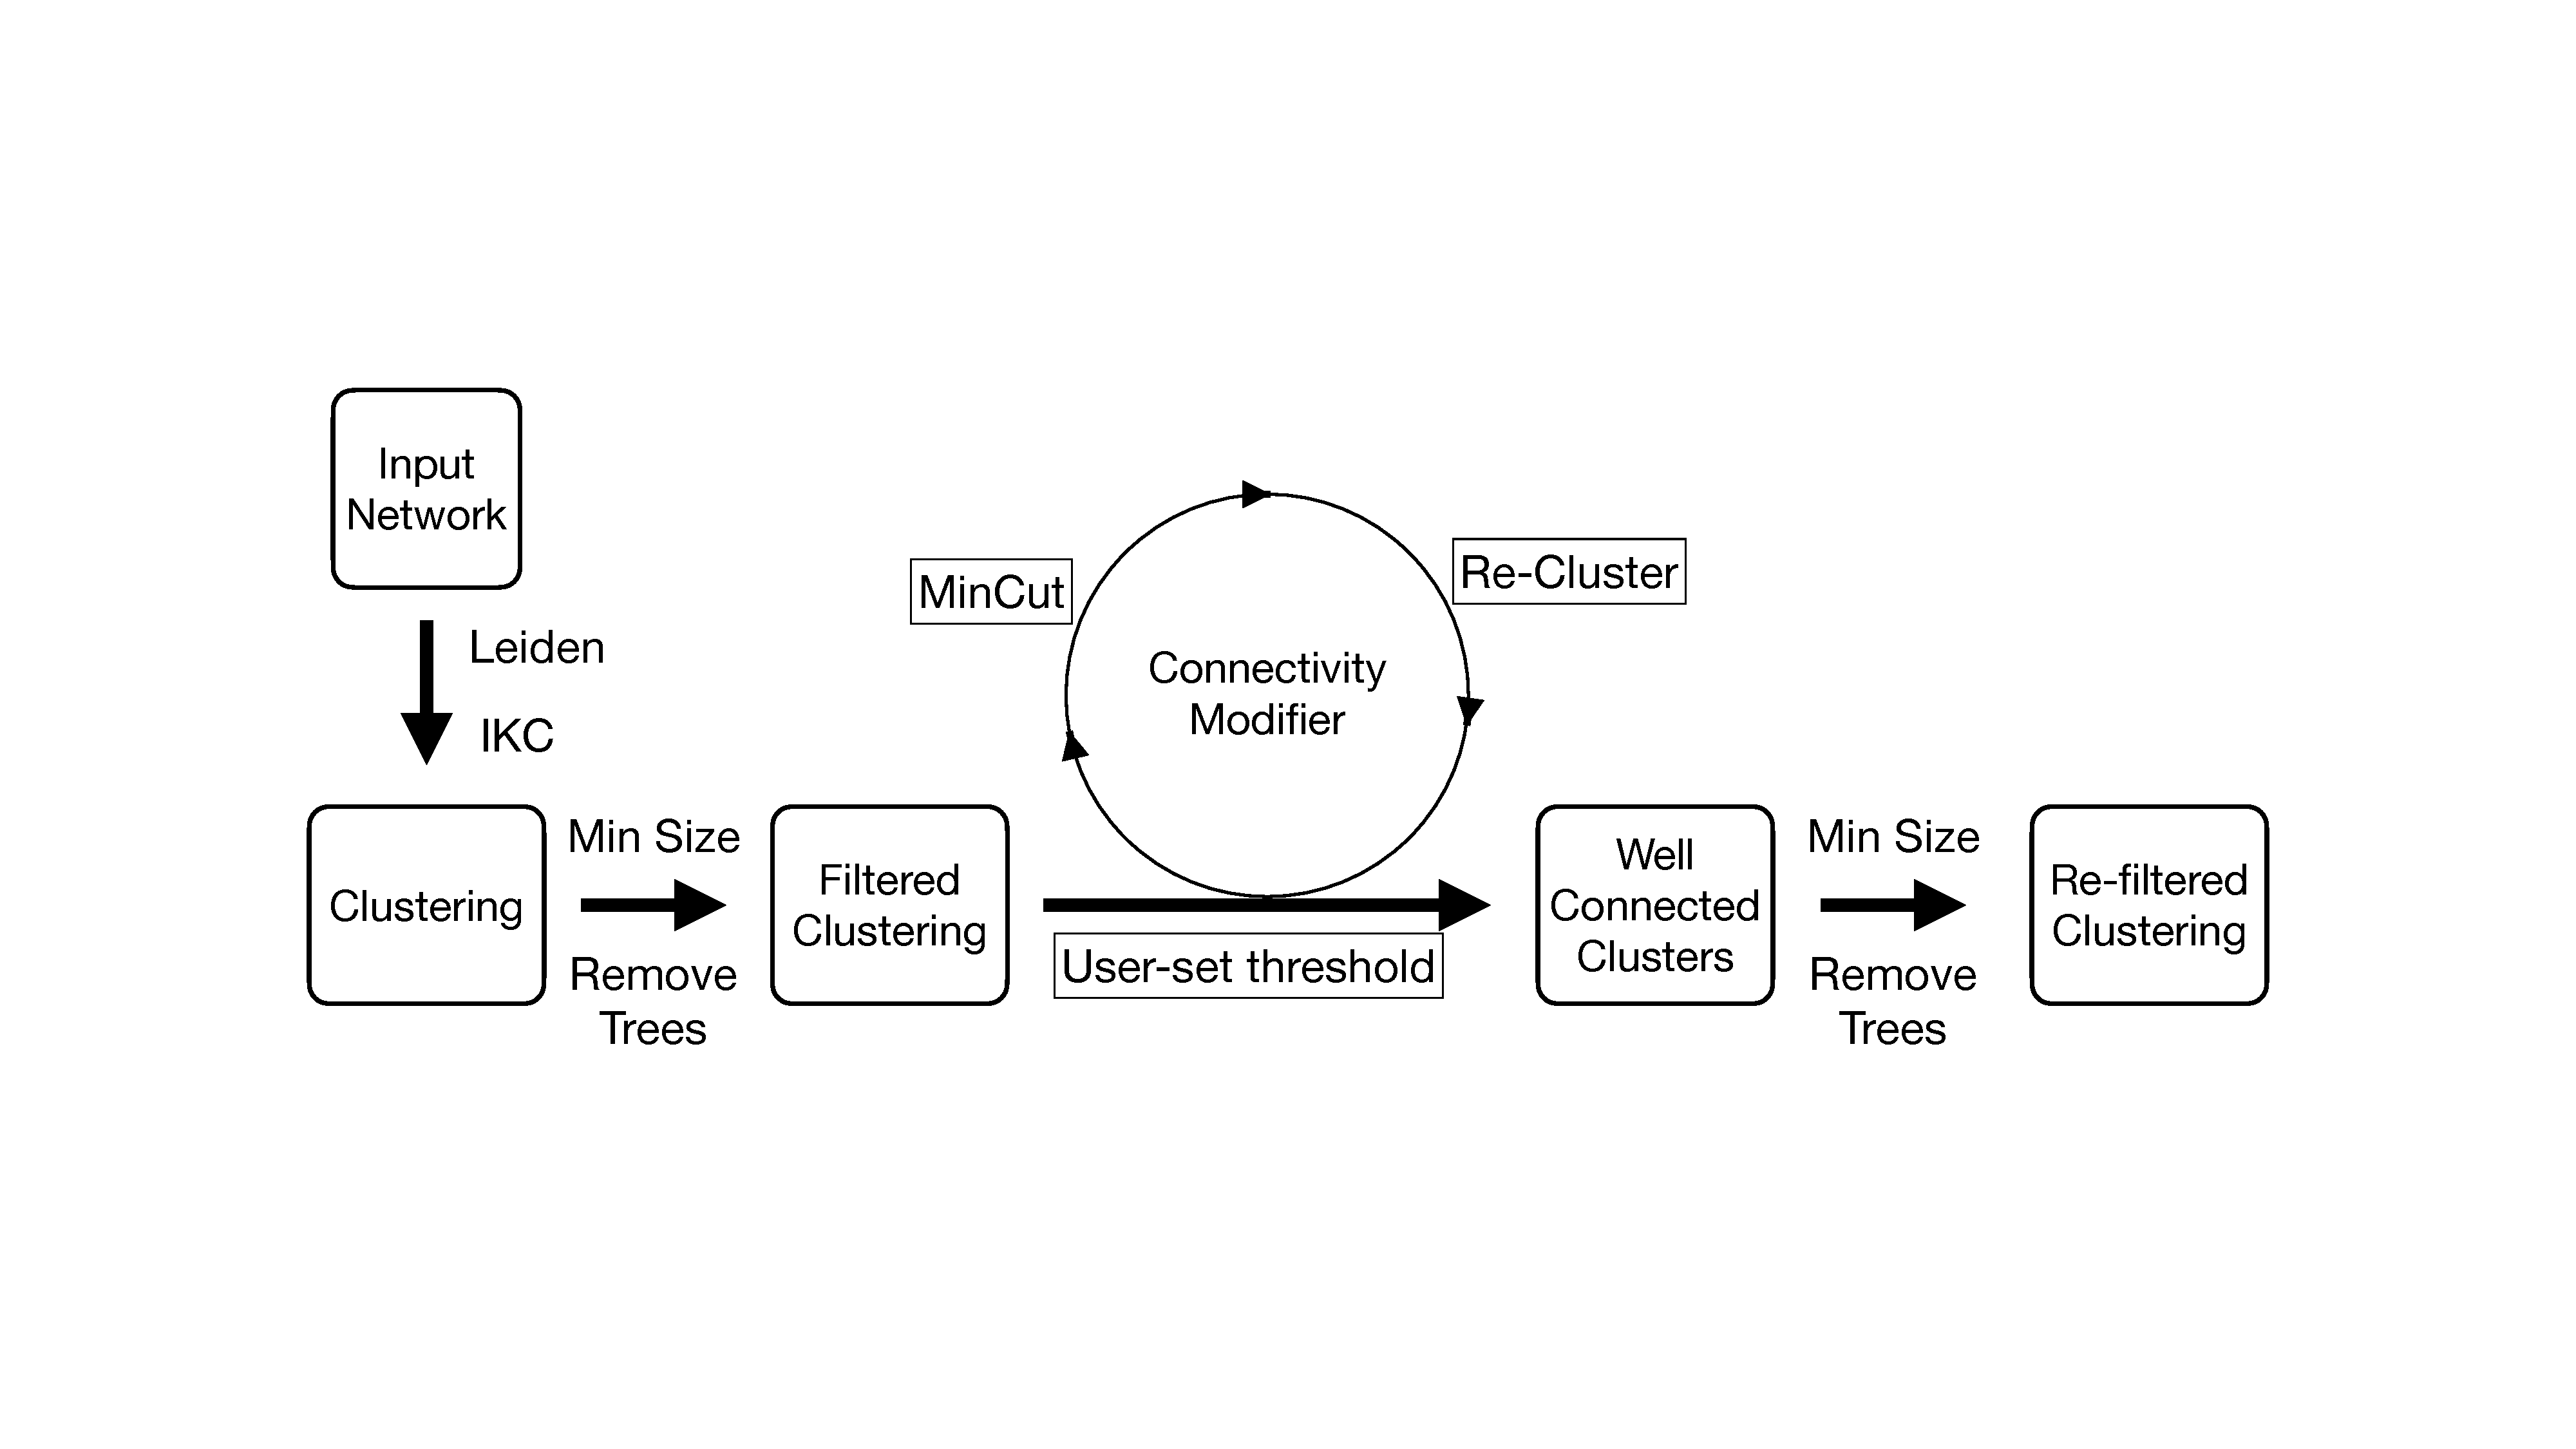
\includegraphics[width=0.8\linewidth]{figs/workflow.pdf}
\caption{Pipeline Schematic. The pipeline depends on user-specified algorithmic parameters (minimum allowed size of a cluster, required minimum number of edges in an edge cut, and clustering method), and operates in four stages:  Stage 1 computes the clustering; Stage 2 removes any clusters that are too small or that are trees;  Stage 3 runs the  Connectivity Modifier to each cluster (i.e., removing small edge cuts if they are below the required size, reclustering, and recursing),  and Stage 4 then removes the clusters that are too small. All clusters that are returned are well-connected by definition and above the minimum size, both algorithmic parameters specified by the user.}
\end{figure}




In this study, we report results using default values for the algorithmic parameters, which are: $B=11$ (so that all clusters of size at most 10 are considered too small) and requiring that the minimum edge cut for a cluster $C$ be at least  $ 1+ \lfloor \log_{10}(||C||) \rfloor$,  where $||C||$ denotes the number of vertices in $C$.
We report results using both Leiden optimizing CPM with different resolution parameter values and IKC, and we explore results on several networks.


\subsubsection{Filters} Clusters were filtered to remove trees and any cluster of size at most 10,. Many tools can achieve this; see supplementary information for details.
%using any of the following tools: (i) a custom R script, (ii) sequential or parallelized Python scripts using the Networkit library \citep{Staudt2016}, or (iii) Belinda, a Python package [cite supplementary information and insert Github reference to https://github.com/illinois-or-research-analytics/belinda] for clustering analysis.

\subsubsection{Connectivity Modifier} To recursively compute and apply minimum cuts to individual clusters, we used the Connectivity Modifier (CM) code at [insert Github reference to Connectivity Modifier], which uses Viecut \citep{Henzinger2018,Henzinger2019} as a dependency, and takes as input a clustering from either the Leiden algorithm or IKC, and returns a set of clusters that is guaranteed to be
well-connected.
We filtered the input clustering as above before passing it as input to Connectivity Modifier. [insert references https://pypi.org/project/connectivity-modifier/].

Here we describe the CM code when passed an input  Leiden clustering $\mathcal{C}$  optimizing CPM (i.e., in default mode). We note that modifying this description to describe how it works with IKC or with Leiden for modularity is straightforward.
We assume that the user has specified the value of the resolution parameter $r$ (referred to as $\gamma$ above and in some publications).
We assume that the minimum size of the edge cut is specified, but recall that our default setting specifies that any edge cut for a cluster $C$ that is at most $ \lfloor \log_{10}(||C||) \rfloor$ is ``too small".
CM used with Leiden and parameter $r$ has the following structure.


First, the set $Bin$ is initialized to the empty set  ($\emptyset$).
CM  then orders the clusters in the input clustering, and   processes each cluster in  turn.
When processing a single cluster $C$,
CM uses VieCut to find a small cut in $C$;  if the cut is too small (i.e., for our default, this means it has at most $\log_{10}(||C||)$ edges), then
we remove the edge cut from the cluster, which splits the cluster $C$ into two  subsets $A$ and $B$.
Both $A$ and $B$ are then reclustered using Leiden with the specified resolution parameter.
Every cluster that results is then recursively analyzed using the same CM pipeline, and the recursion stops when each cluster is considered well-connected.
All the clusters that are produced by this process are therefore well-connected, and are placed in the set $Bin$.

After all clusters are processed, the set $Bin$ is returned.
By design, every cluster in  $Bin$ will be well-connected (i.e., the min cut found using VieCut will be large enough, according to the user-specified criterion).
Furthermore, every cluster in the output will either be one of the input clusters or will be a subset of one of the input clusters.
Finally, every cluster in the input that meets the user-specified criteria for size and edge-connectivity will be found in $Bin$.

\begin{figure}[H]
\centering
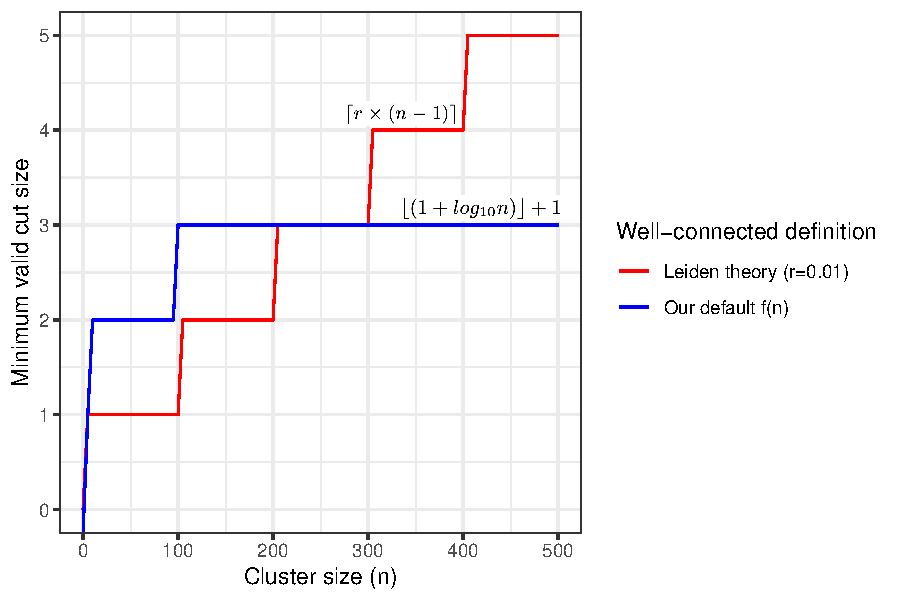
\includegraphics[width=0.7\linewidth]{figs/well_connected_definition.pdf}
\caption{Comparison of  the  lower bounds for well-connected clusters,  given in Equations \ref{eqn:cpm-bound} and \ref{eqn:our-bound}.
Equation \ref{eqn:cpm-bound} depends on the sizes of the two subsets formed by deleting the edge-cut; what we show here is based on the most imbalanced split (i.e., separating a single node from the remaining nodes in the cluster).
The figure shows two curves: the red one is for Equation \ref{eqn:cpm-bound} using $r=0.01$ and the blue one is for Equation \ref{eqn:our-bound}.
Accordingly, we see that a cluster with 200 nodes whose minimum cut is of size two, separating one node from the remaining 199 nodes, is considered well-connected
according to Equation \ref{eqn:cpm-bound}  but not according to Equation \ref{eqn:our-bound}.  However, once the cluster exceeds size 300, the lower bound for being well-connected according to
Equation \ref{eqn:cpm-bound}   is larger than the lower bound according to Equation \ref{eqn:our-bound}, making
Equation \ref{eqn:cpm-bound} a ``higher standard".
Thus, the two definitions of ``well-connected"  are meaningful in different
regions of cluster size, with Equation \ref{eqn:cpm-bound}  a higher standard on large clusters (here, above size 301) and Equation \ref{eqn:our-bound}   a higher standard on small to moderate-sized clusters (below 201).
Recall that Equation \ref{eqn:cpm-bound}  defines the lower bound for an edge cut separating one node from the remaining $n-1$ nodes
  in a cluster with $n$ vertices of $\lceil r \times (n-1) \rceil$, where $r$ is the resolution parameter (here, $r=0.01$)
and Equation \ref{eqn:cpm-bound} defines the lower bound on the cut size of $\lfloor(1 + log_{10}n)\rfloor +1$.}
\end{figure}

 \subsection{Data} Several networks were used for testing and analysis and were selected to provide a range of origin, size and edge density. In all cases, below the counts of nodes and edges are reported after removing duplicate records,
self-citations, and parallel edges from the source data.

\paragraph{Open Citations}
A custom-implemented ETL process was designed to process the publicly available OpenCitations dataset \citep{Peroni2020} and load it into a PostgreSQL table. Citation data was downloaded in Aug 2022. A custom ETL script, written in Bash and SQL, was used to find and pipe uncompressed CSV files, in 20 parallel jobs using the GNU Parallel command-line utility, to a custom function which loaded individual CSV files into a staging view. DOIs were also checked for case differences to remove duplicates.  The resultant network contained 75,025,194 nodes and 1,363,605,603 edges.


\paragraph{Curated Exosome Network (CEN)}
The CEN is a citation network focused on the exosome research literature consisting of 13,989,436 nodes and 92,051,051 edges. Its construction has previously been previously described in \cite{Jakatdar_2022}.


\paragraph{SNAP Networks}The following networks were downloaded from the Stanford Network Analysis Project (SNAP) website: (i) cit\_patents \citep{Leskovec2005}, a citation network among US patents, (ii) orkut \citep{Yang2013}, data from the Orkut online social network, (iii) cit\_hepph \citep{Leskovec2005}, the Arxiv High Energy Physics paper citation network,  (iv) wiki\_talk \citep{Leskovec2010}, a network containing users and discussion from the inception of Wikipedia till January 2008, (v) wiki\_topcats \citep{Yin2017}, a web graph of Wikimedia hyperlinks. Each network was processed to remove duplicate edges, parallel edges, and self-loops.
The numbers of nodes and edges reported in Table \ref{tab:empirical-stats-SNAP} reflect this processing.

\begin{table}[ht]
\centering
\begin{tabular}{lrrr}
  \hline
 network & edges & nodes & avg\_deg \\
  \hline
  cit\_hepph & 420,877 & 34,546 & 24.37 \\
  cit\_patents & 16,518,947 & 3,774,768 & 8.75 \\
  orkut & 117,185,083 & 3,072,441 & 76.28 \\
  wiki\_talk & 4,659,565 & 2,394,385 & 3.89 \\
  wiki\_topcats & 25,444,207 & 1,791,489 & 28.41 \\
   \hline
\end{tabular}
% Counts manually verified on Jan 31. 2023 by gc
\caption{Empirical statistics for cleaned versions of 5 SNAP networks.}
\label{tab:empirical-stats-SNAP}
\end{table}

\paragraph{LFR (random) networks}

We used the LFR benchmark graphs from \cite{lancichinetti2008benchmark} to create simulated networks with ground truth communities, while attempting to emulate the properties of each empirical network and its corresponding Leiden clustering. The generative model of the LFR graphs assume that the node degree and the community size distributions are power-law distributions, a property that is usually seen in large real networks \citep{albert2002statistical}.

The software for generating LFR benchmark graphs\footnote{available at \href{https://www.santofortunato.net/resources}{https://www.santofortunato.net/resources}} takes the following eight parameters as input:
\begin{itemize}
    \item  \textbf{Node properties:} Number of nodes $N$, average and maximum node degrees ($k$ and $k_{max}$ respectively), and exponent for degree sequence ($\tau_1$) that is assumed to be a power-law.
    \item \textbf{Community properties:} Maximum and minimum community sizes ($c_{max}$ and $c_{min}$), and minus exponent for the community size distribution ($\tau_2$), also modeled as a power-law.
    \item Mixing parameter $\mu$, that is the ratio between the degree of a node outside its community and its total degree, averaged over all nodes in the network. Lower $\mu$ values suggest that the network is constituted from well-separated communities, as nodes are mostly connected to other nodes inside their communities, rather than outside of it.
\end{itemize}






\paragraph{Parameter Estimation.} To emulate real networks using LFR graphs, we estimated all eight parameters described above for a given pair of network $\mathcal{G}$ and a clustering $\mathcal{C}$. Computing $N, k, k_{max}, c_{min}$ and $c_{max}$ is straightforward using \texttt{networkX} \citep{hagberg2008exploring}. To estimate $\mu$, we do a single iteration over all edges of the network, and for each edge, if the nodes on the two sides of it were in different communities, that edge contribute to the ratio $\mu$ of these two nodes. The total $\mu$ of the network/clustering pair is the average $\mu$ of all nodes.

To estimate $\tau_1$ and $\tau_2$, we fit a power-law distribution to the node degree sequence and the community size distribution, using the approach from \cite{clauset2009power} that is implemented in the \texttt{power-law} Python package \citep{alstott2014powerlaw}. Note that the power-law property may hold for the \textit{tail} of the degree or community size sequence and not the whole distributions. Therefore, following \cite{clauset2009power}, we estimate $x_{min}$, the minimum value for which the power-law property holds as well as the exponent $\alpha$ for the tail of the distribution. Our script for estimating these parameters is available at \href{https://github.com/illinois-or-research-analytics/cm_manuscript/tree/main/analysis/lfr-analysis}{https://github.com/illinois-or-research-analytics/cm\_manuscript/tree/main/analysis/lfr-analysis}.


\begin{table}[ht]
\caption{Empirical statistics for LFR networks resembling the OpenCitations, CEN and 4 of the SNAP networks. The resolution parameter used for generating the LFR graphs shown in this table is 0.01.}
\centering
\begin{tabular}{lrrr}
  \hline
 network & nodes & edges & avg\_deg \\
  \hline
    LFR-open\_citations & 3,000,000  & 55,135,215 & 36.76 \\
    LFR-cen & 3,000,000 & 20,762,221 & 13.84 \\
    LFR-cit\_hepph &  34,546 & 431,127 & 24.95 \\
    LFR-cit\_patents & 3,774,768 & 15,640,122 & 8.29 \\
    LFR-wiki\_talk & 2,394,385 & 3,297,391 & 2.75 \\
    LFR-wiki\_topcats & 1,791,489 & 24,494,292 & 27.34 \\
 \hline
\end{tabular}
\label{tab:empirical-stats-LFR}
\end{table}
\paragraph{Generating LFRs.} After computing these parameters based on the Leiden clusterings of the empirical networks using selected resolution parameters (see text), we simulated LFR networks using the software from \citep{lancichinetti2008benchmark}, producing empirical statistics reported in Table \ref{tab:empirical-stats-LFR} (for a resoution parameter of 0.01). For networks with more than 10 million nodes, i.e. the OpenCitations and the CEN, we limited the number nodes to 3,000,000, due to scalability limitations of LFR benchmark graph generator \citep{slota2019scalable}, while persevering the density (reflected by average degree) and the mixing parameter. For the rest of the networks, the number of nodes of the LFR graph exactly matches the number of nodes in the corresponding empirical network. In some cases, due to the inherent limitations of the LFR graph generator, we had to modify the ranges of the community sizes (i.e. increase $c_{min}$ and decrease $c_{max}$) to generate the network. For the Orkut network, which is very dense with an average node degree of 76.28, we were not able to generate a corresponding LFR even after examining a wide range of parameter values and relaxing the bounds on the degree and community size distirbutions. For the rest of the networks however, as shown from the statistics reported in Table \ref{tab:empirical-stats-LFR} and the supplement \textcolor{blue}{add table number}, the average node degree, the mixing parameter and the exponents for the degree and community size distributions are in all cases very well-preserved. Further details about the pipeline for producing LFR graphs and the statistics of the graphs are provided in Supplementary Materials Sec. 2.

\section{Experimental Design}
\label{sec:expt-design}
We ran a sequence of experiments, in each case clustering networks using Leiden under CPM-optimization and with various parameter values. For some experiments we also ran the IKC pipeline.  In all cases, we explore the impact of the CM pipeline.
\begin{itemize}
\item Experiment 1: We analyze the Open Citations Network using Leiden  and IKC (k=10), followed by the CM pipeline.
\item Experiment 2: We analyze the Curated Exosome Biology (CEN) network using Leiden and IKC, followed by the CM pipeline.
\item Experiment 3: We analyze LFR networks built to resemble the Open Citations Network and the CEN network (using Leiden clusterings), using Leiden, followed by the CM pipeline.
\item Experiment 4: We analyze networks from the SNAP collection and their LFR model networks, in each case using Leiden followed by the CM pipeline.
\end{itemize}

For each experiment, we report empirical statistics, such as the distribution of cluster sizes, node and edge coverage (both for clusters that are of size at least 2 and of size at least 10), and percentage of clusters that fail each of our ``valid community" tests (i.e., being at least size 11 and being well-connected according to Equation \ref{eqn:our-bound}).

\section{Results and Discussion}
\label{sec:results-discussion}

\subsection{Experiment 1: Analyses of the Open Citations Network}

\begin{figure}[H]
\centering
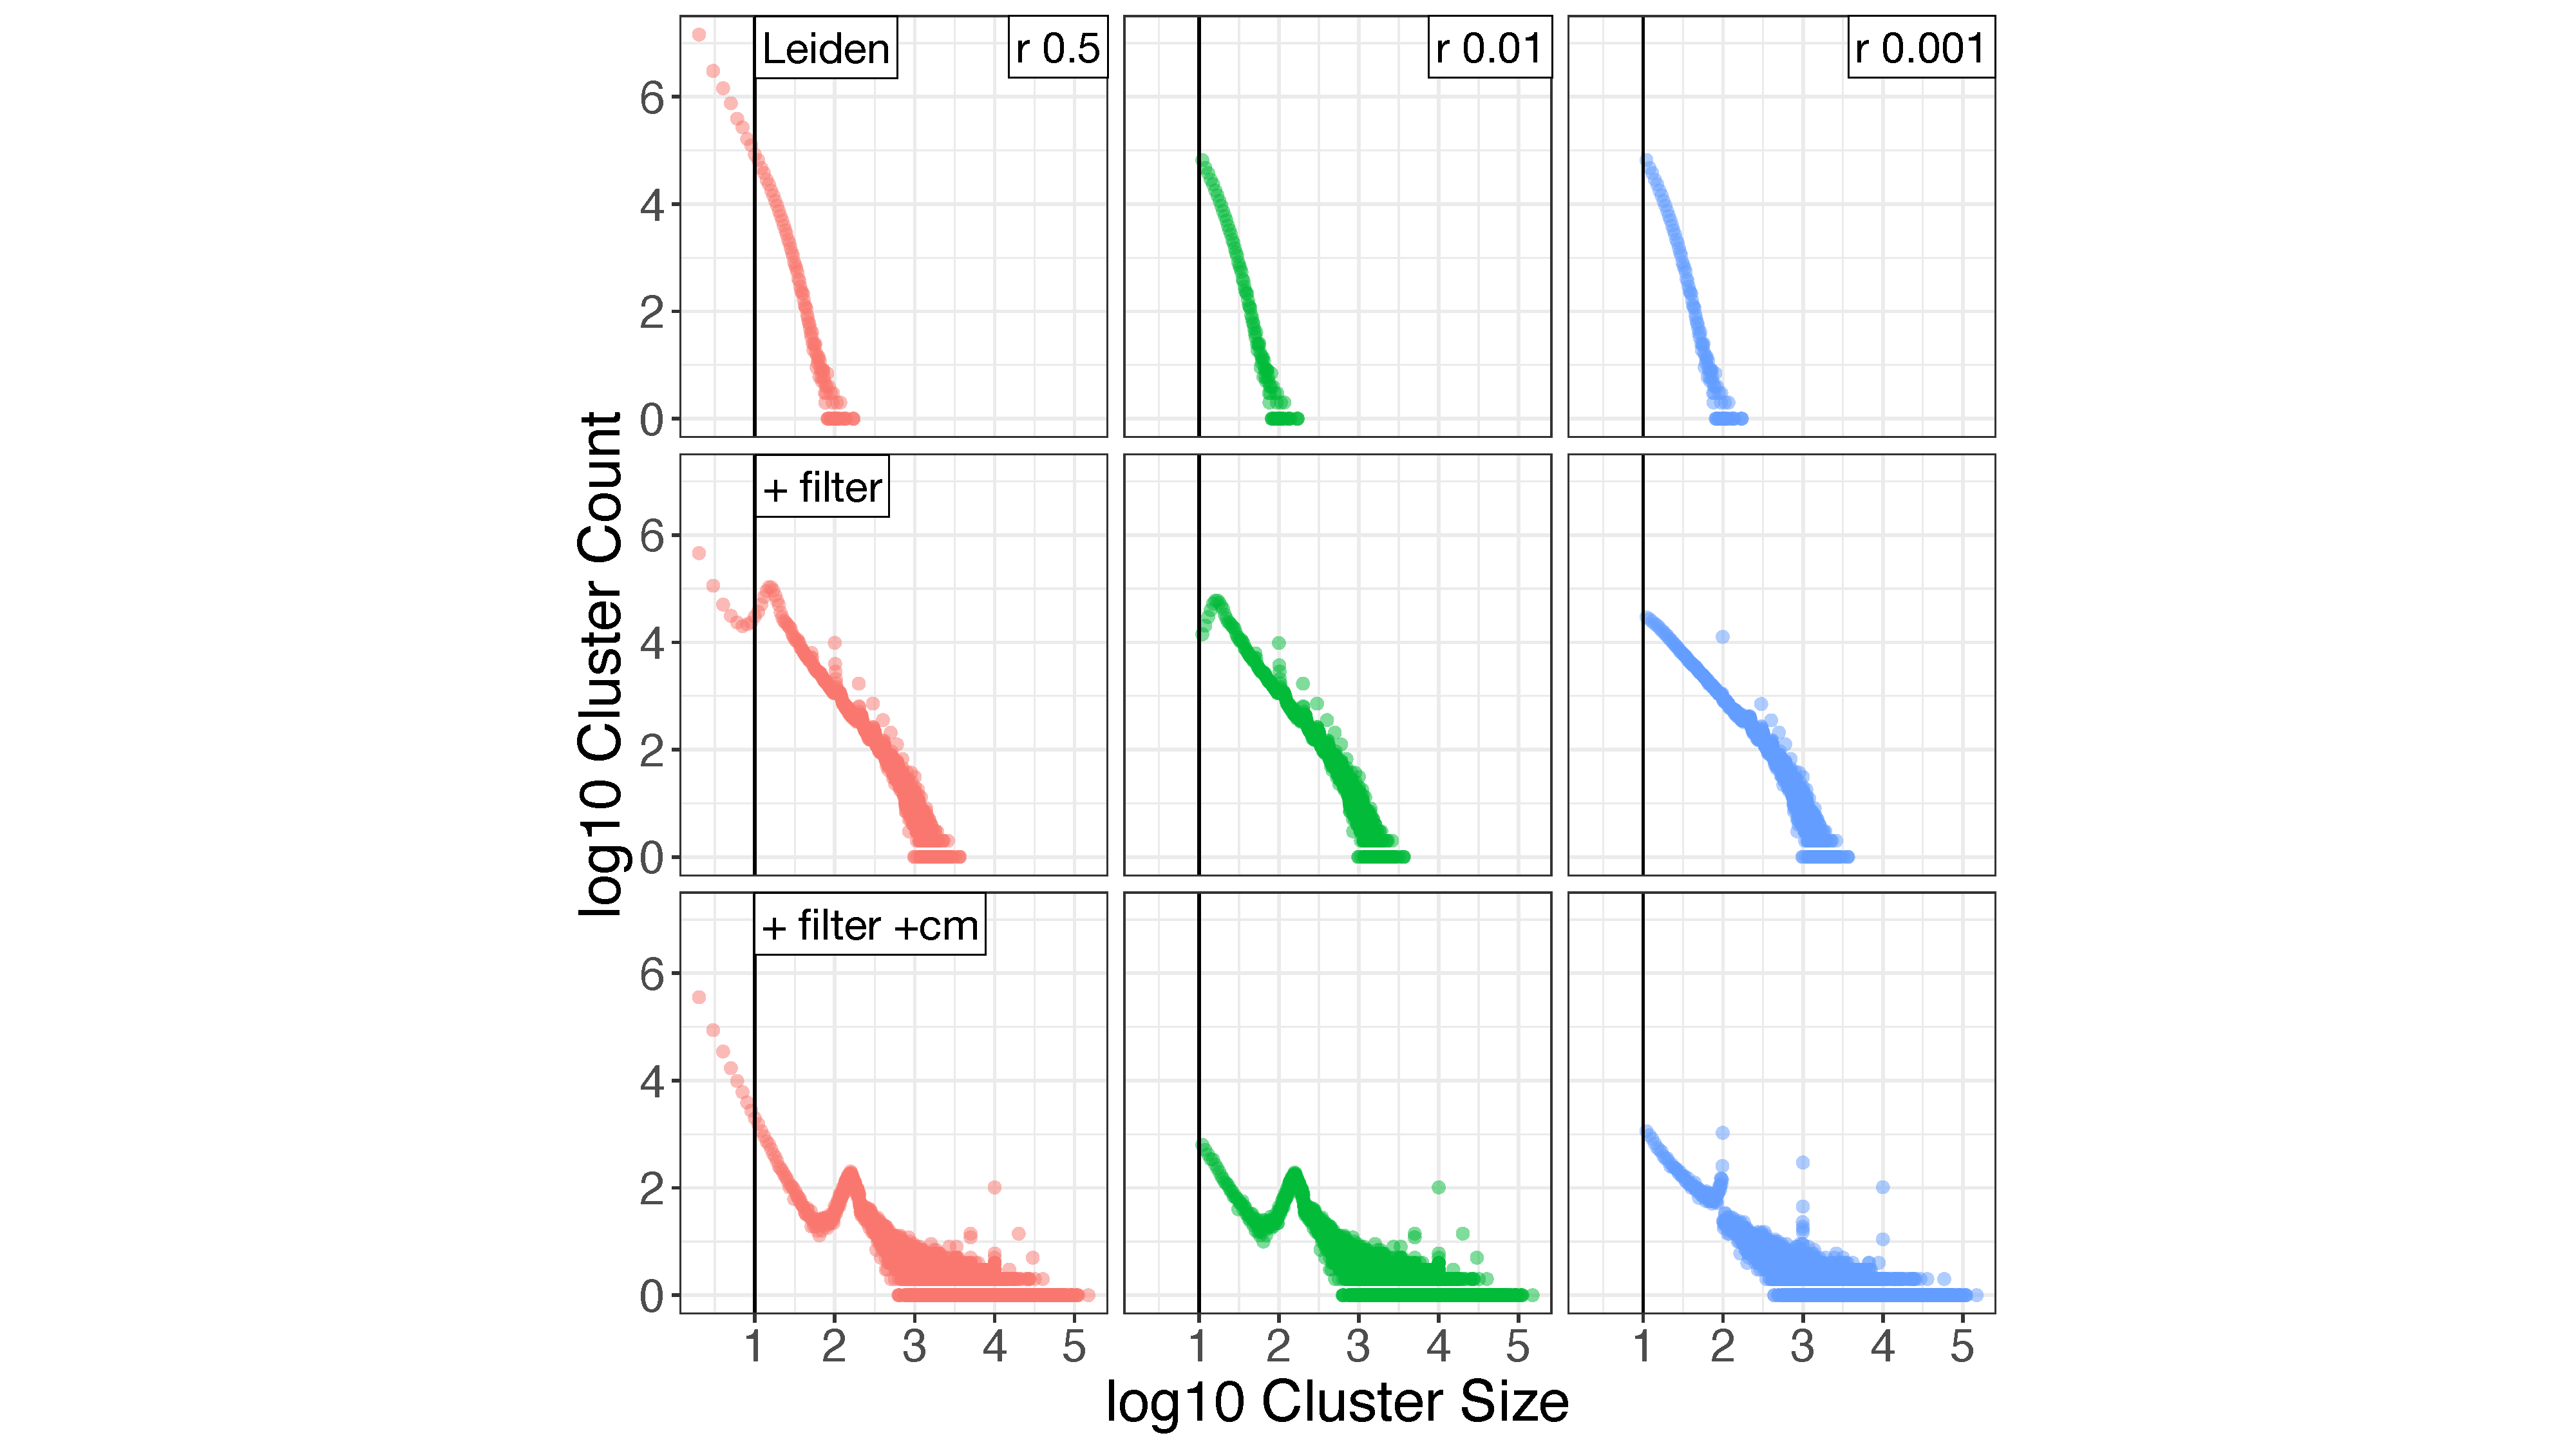
\includegraphics[width=0.8\linewidth]{figs/fig1_kn.pdf}
\caption{Connectivity modifier (CM)-processed Leiden clusterings of the Open Citations network exhibit a resolution-dependent reduction in clusters and cluster sizes.
The Open Citations network consisting of 75,025,194 nodes and 1,363,605,603 edges was clustered using the Leiden algorithm, with CPM as quality function; each row shows results for a particular resolution value (top: r=0.5, middle: r=0.01, bottom: r=0.0001).
The first column shows the cluster size distribution for the Leiden clustering; the middle column shows the cluster size distribution after filtering out trees and clusters of size at most 10; the right column shows the cluster size distribution after the complete CM pipeline (which includes a final filtering step to remove trees and clusters at most size 10).
The impact on Leiden clustering is largest for the two smaller resolution values.
%The effect of filtering out tree clusters and clusters of size 10 or less and trees is shown in the middle column. The effect of subsequent treatment with CM and re-filtering is shown in the the right column.
Descriptive statistics are shown for Leiden clustering of this network at 5 different resolution values in Table \ref{tab:something}.}
\label{fig:oc_size_count_plots}
\end{figure}

% latex table generated in R 4.1.3 by xtable 1.8-4 package
% Sun Feb 26 21:54:10 2023
\begin{table}[H]
\centering
\begin{tabular}{rllrrrrr}
  \hline
 & res & Rx & clus\_count & node\_cov & min & median & max \\
  \hline
1 & Leiden 0.5 & cluster & 20964020 & 79.2 &   2 & 2. & 172 \\
  2 & Leiden 0.5 & filter & 297755 & 6.0 &  11 & 13 & 172 \\
  3 & Leiden 0.5 & cm & 297755 & 6.0 &  11 & 13. & 172 \\
  \hline
  4 & Leiden 0.1 & cluster & 8642592 & 92.8 &   2 & 5 & 882 \\
  5 & Leiden 0.1 & filter & 1296921 & 43.5 &  11 & 17 & 882 \\
  6 & Leiden 0.1 & cm & 1167461 & 41.6 &  11 & 19 & 882 \\
  \hline
  7 & Leiden 0.01 & cluster & 2135152 & 92.4 &   2 & 15 & 3678 \\
  8 & Leiden 0.01 & filter & 1033288 & 82.2 &  11 & 24 & 3678 \\
  9 & Leiden 0.01 & cm & 579753 & 64.0 &  11 & 30 & 3678 \\
  \hline
  10 & Leiden 0.001 & cluster & 840081 & 92.7 &   2 & 3 & 22808 \\
  11 & Leiden 0.001 & filter & 208192 & 89.3 &  11 & 73 & 22808 \\
  12 & Leiden 0.001 & cm & 145954 & 68.7 &  11 & 64 & 22808 \\
  \hline
  13 & Leiden 0.0001 & cluster & 560234 & 93.7 &   2 & 2 & 149287 \\
  14 & Leiden 0.0001 & filter & 33763 & 91.7 &  11 & 206 & 149287 \\
  15 & Leiden 0.0001 & cm & 27666 & 68.0 &  11 & 91 & 149287 \\
   \hline
\end{tabular}
\caption{Clustering Open Citations with the Leiden algorithm at five different resolution values. For each resolution value, the number of non-singleton clusters, and node coverage (count of nodes in clusters expressed as a percentage of the total number of nodes in the network. \emph{Filter} indicates that clusters of size $<=10$ and tree clusters have been removed. \emph{cm} indicates that the recursive mincut and cluster connectivity modifier process was applied to the filtered clusters followed by refiltering to exclude clusters of size at most 10.}
\label{tab: cm_stats}
\end{table}

\begin{table}[H]
\centering
\begin{tabular}{lrrrrrr}
  \hline
 clustering & res\_value & clus\_count & node\_cov & min & med & max \\
  \hline
Leiden & 0.5 & 297038 & 5.98 &  11 & 13.00 & 183 \\
Leiden & 0.1 & 1313856 & 43.78 &  11 & 17.00 & 882 \\
Leiden & 0.01 & 1361168 & 88.93 &  11 & 19.00 & 3530 \\
Leiden & 0.01 & 232288 & 90.56 &  11 & 64.00 & 23470 \\
Leiden & 0.0005 & 133147 & 90.97 &  11 & 90.00 & 39049 \\
Leiden & 0.0001 & 39069 & 91.81 &  11 & 177.00 & 176557 \\
   \hline
\end{tabular}
\caption{Clustering the Open Citations Network. The Open Citations Network (Materials and Methods) consisting of 75,025,194 nodes and 1,363,605,603 edges was clustered with the Leiden algorithm, using the Constant Potts Model (CPM) as quality function, and using various resolution values (column 1). Node coverage is expressed as the the percent of nodes in these clusters of size greater than 10 relative to the total number of nodes in the network. Minimum, median, and max cluster sizes are shown in the last three columns.  }
\end{table}


\subsection{Experiment 2: Analyses of the Curated Exosome Network (CEN)}

We then evaluated a citation network, the CEN (Materials and Methods) consisting of 13,989,436 nodes and 92,051,051 edges, which captures the relatively recent literature relevant to exosomes and extracellular vesicles. We clustered the CEN using Leiden optimizing CPM with resolution values ranging from 0.5 to 0.001 (Table \ref{tab:CEN-table1}). This range of resolution values brackets the resolution values used by us on this network in earlier studies \citep{Wedell2022,Jakatdar_2022}.

% latex table generated in R 4.1.3 by xtable 1.8-4 package
% Mon Jan 30 22:29:28 2023
% generated by singleton corrected script.
\begin{table}[ht]
\centering
\begin{tabular}{rlrrrrrrr}
  \hline
 & clustering & n=1 & n$>$1 & n$>$10 & min & med & max & node\_cov \\
  \hline
1 & leiden 0.5 & 12,701,653 & 433,557 & 8,503 & 11 & 14 & 68 & 0.97 \\
  2 & leiden 0.1 & 8,341,818 & 516,299 & 273,420 & 11 & 11 & 319 & 23.98 \\
  3 & leiden 0.01 & 3,245,556 & 280,518 & 275,641 & 11 & 28 & 3,186 & 76.52 \\
  4 & leiden 0.001 & 2,172,927 & 66,326 & 65,771 & 11 & 98 & 16,481 & 84.45 \\
   \hline
\end{tabular}
\caption{Clustering the Curated Exosome Network (CEN) with Leiden. Node coverage and cluster size increase as resolution values is decreased. The first column (clustering) shows the resolution value passed as a parameter to Leiden. The next three columns show cluster counts for singleton clusters, non-singleton clusters, and clusters of size at least 11. Minimum, median, and max cluster sizes are shown for clusters of size at least 11. The last column indicates node coverage expressed as a percentage; the count of nodes in clusters of size at least 11, relative to the total number of nodes in the network.}
\label{tab:CEN-table1}
\end{table}

Predictably, node coverage increased as resolution values was decreased. Of interest, however, was whether trees, which are excellent examples of poorly connected clusters, were being generated. Accordingly, we searched for trees in clusterings generated by either Leiden or IKC. In both cases, we filtered out clusters of size $10$ or less before evaluating clusters for the presence of trees. Strikingly, we observed trees in Leiden clusterings from resolution values of 0.1, 0.01, and 0.001 but not at 0.5. At resolution value of 0.1, 273,420 clusters were generated of which 254,734 (93.2\%) were trees of size 11. At a resolution value of 0.001, 65,771 clusters were generated were found of which 22,750 (34.6\%) were
trees (Figure \ref{fig:trees-in-networks} and Table \ref{tab:CEN-table2}. Interestingly, as resolution values were decreased further, the number of trees decreased but the average tree size increased (Figure \ref{somefig}, Table \ref{tab:CEN-table3}).

\begin{figure}[h]
\centering
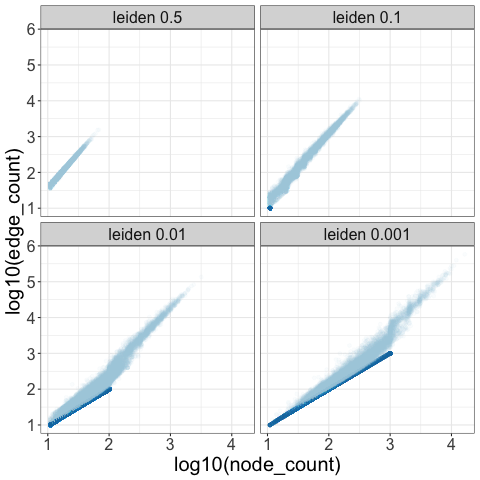
\includegraphics[width=0.4\linewidth]{figs/cen_quad_fig1.png}
\caption{The CEN was clustered at four resolution values (0.5, 0.1, 0.01, 0.001) using the Leiden algorithm.
%with CPM as quality function.
The figure shows the count of nodes in each cluster of size greater than 10 plotted against the count of nodes in each cluster (cluster size); dark blue indicates tree clusters.
As resolution value decreases, node coverage (the fraction of nodes that are found in clusters of size $>$  10) increases. The number of such clusters does not, however, monotonically increase (Table \ref{tab:CEN-table1}). As the resolution value decreases, tree clusters are detected, with maximum tree size inversely related to resolution value. However, the number of trees decreases as the resolution factor is decreased, with the exception of clustering at 0.5 for which no trees are detected (Table \ref{tab:CEN-table2}).}
%The Curated Exosome Network (CEN) consists of 13,989,436 nodes and 92,051,051 edges. The average degree of its nodes is 13.16.
\end{figure}

To follow up on the presence of sparse clusters in the form of trees, Leiden clusters were filtered to exclude clusters of size at most 10, after which the number of clusters that were \emph{trees} (ti.e., clusters that have no cycles, equivalently the case where he number of nodes in a cluster is exactly  one more than the number of intra-cluster edges) were counted. Trees were then filtered, after which the remaining clusters were processed with connectivity modifier (CM) using Equation \ref{eqn:our-bound} as the threshold, then filtered again to remove small clusters (Table \ref{tab:CEN-table2}).

% latex table generated in R 4.1.3 by xtable 1.8-4 package
% Sun Jan 29 23:08:57 2023
% generated by running table2.R on odesa in
% /data1/snap_leiden_venv/cen

\begin{table}[H]
\centering
\begin{tabular}{rllrrrrr}
  \hline
 & clustering & rx & cluster\_count & min & median & max & node\_cov \\
  \hline
1 & leiden.5 & -  & 8503 &  11 & 14.00 &  68 & 0.97 \\
  2 & leiden.5 & filter & 8503 &  11 & 14.00 &  68 & 0.97 \\
  3 & leiden.5 & cm & 8503 &  11 & 14.00 &  68 & 0.97 \\
  4 & leiden.5 & filter & 8503 &  11 & 14.00 &  68 & 0.97 \\
  5 & leiden.1 & - & 273420 &  11 & 11.00 & 319 & 23.98 \\
  6 & leiden.1 & filter & 18686 &  11 & 20.00 & 319 & 3.95 \\
  7 & leiden.1 & cm & 14681 &  11 & 20.00 & 319 & 3.63 \\
  8 & leiden.1 & filter & 14681 &  11 & 20.00 & 319 & 3.63 \\
  9 & leiden.01 & -& 275641 &  11 & 28.00 & 3186 & 76.52 \\
  10 & leiden.01 & filter & 64320 &  11 & 34.00 & 3186 & 24.80 \\
  11 & leiden.01 & cm & 34071 &  11 & 24.00 & 3186 & 13.20 \\
  12 & leiden.01 & filter & 34071 &  11 & 24.00 & 3186 & 13.20 \\
  13 & leiden.001 & - & 65771 &  11 & 98.00 & 16481 & 84.45 \\
  14 & leiden.001 & filter & 43021 &  12 & 112.00 & 16481 & 62.31 \\
  15 & leiden.001 & cm & 27581 &  11 & 32.00 & 16480 & 23.15 \\
  16 & leiden.001 & filter & 27581 &  11 & 32.00 & 16480 & 23.15 \\
   \hline
\end{tabular}
\caption{Identifying well connected clusters from Leiden clustering of the CEN. For each of resolution values \{0.5, 0.1, 0.01, 0.001\}, clusters were limited to those of size 11 or greater, then depleted of trees, the processed by CM, and then filtered to remove any clusters of size 10 or less as well as trees. Node coverage is least 0.5 and at most  0.01 (Table \ref{tab:CEN-table1}. However, removal of trees and CM treatment reduces node coverage by 20.4\%, 63.3\%, and 61.3\% of the original values for resolution values of 0.01, 0.01, and 0.001 respectively.  For example, at resolution value 0.001, node coverage drops from 84.45\% to 23.15\%. At a resolution value of 0.5, no change is observed.}
\label{tab:CEN-table2}
\end{table}


% latex table generated in R 4.2.2 by xtable 1.8-4 package
% Sun Jan 15 17:37:03 2023
\begin{table}[H]
\centering
\begin{tabular}{lrllrrr}
  \hline
 Clustering & Resolution & type & min & med & max \\
  \hline
leiden & 0.5 & non\_tree &  11 & 14 &  68 \\
leiden & 0.5 & tree &  NA & NA &  NA \\
leiden & 0.1 & tree &  11 & 11 &  11 \\
leiden  & 0.1 & non\_tree &  11 & 20 & 319 \\
leiden  & 0.01 & tree &  11 & 27 & 101 \\
leiden & 0.01 & non\_tree &  11 & 34 & 3186 \\
leiden & 0.001 & tree &  11 & 65 & 1001 \\
leiden & 0.001 & non\_tree &  12 & 112 & 16481 \\

   \hline
\end{tabular}
\caption{Cluster sizes for Leiden clusters on the CEN. We show empirical statistics (minimum, median, and maximum) of Leiden clusters generated using the Constant Potts Model (CPM) as quality function and with different resolution values. Clusters of of size at most 10 have been removed. Do we need this table?}
\end{table}

% latex table generated in R 4.2.2 by xtable 1.8-4 package
% Fri Jan 13 18:03:02 2023


\textcolor{blue}{Insert Minhyuk's IKC data for CEN}.


\subsection{Experiment 3: Analyses of LFR networks based on the Open Citations and CEN networks}

\subsection{Experiment 4: Analyses of SNAP networks and their LFR model networks}



\section{Conclusions}

\section*{Competing Interests} \vspace{3mm} The authors have no competing interests.

\section*{Funding Information} Research in this manuscript was supported by a partnership between the Insper Institute, Brazil and the Department of Computer Science at the University of Illinois Urbana-Champaign. Roughly
50\% of the work was performed in the Oracle Cloud Infrastructure, courtesy of an Oracle Research Award to Tandy Warnow.

\section*{Data Availability}

\section*{Acknowledgments} We thank Christine Ballard, Bryan Barker, and Nathan Bryans from Oracle for their help in setting up and managing a computational environment in the Oracle Cloud Infrastructure.

\bibliographystyle{apalike}
\bibliography{cmv1}
\end{document}


\begin{itemize}
\item For  the CEN and  for the Open Citations networks, produce one LFR network  that has a mixing parameter and other
parameters set so as to produce something that resembles the given Leiden clustering of the given real-world network. (However, keep the LFR network
on the moderate size, so at most 3,000,000 vertices.)

\item
For each LFR network:
\begin{itemize}
\item Report empirical statistics of the network
\item Report empirical statistics of the true clustering
\item Capture accuracy relative to `ground' truth
\item
Recluster using Leiden (same resolution value) and then run the CM pipeline.
Record all the usual statistics
\item Run CM on the true clustering.
Report all the usual statistics
\end{itemize}
\end{itemize}


\noindent
The usual statistics are things like:
\begin{itemize}
\item Statistics before running the CM pipeline, including distribution of cluster sizes, node and edge coverage. \textcolor{red}{node coverage should be defined somewhere. if it has two definitions (nodes in non-singleton clusters, nodes in clusters with size more than 10), mention both. }

\item Statistics at each stage of the CM pipeline (percentage of clusters that are deleted due to being trees,
then deleted due to being too small, then the percentage of remaining clusters  that have small edge cuts).
But at the end of the pipeline we also remove small clusters.
Also show total node and edge coverage at the end of each stage of the CM pipeline.
\item
In essence we want to know which clusters in the input survive the entire process, which ones are modified.
We'll want their sizes as well, so we can say things like ``20\% of the input clusters above size 100 have small edge cuts" and
``10\% of the input clusters above size 50 are trees".
\end{itemize}


% latex table generated in R 4.1.3 by xtable 1.8-4 package
% Sun Jan 22 19:56:56 2023
\begin{table}[ht]
\centering
\resizebox{.5\textwidth}{!}{
\begin{tabular}{rrrrrll}
  \hline
 & clus\_count & min & med & max & type & gp \\
  \hline
1 & 20648920 &   2 &   2 &  10 & size 2-10 & leiden.5 \\
  2 & 297038 &  11 &  13 & 183 & size $>$10 & leiden.5 \\
  3 & 297038 &  11 &  13 & 183 & non\_tree & leiden.5 \\
  4 & 10349 &  11 &  13 &  85 & pre-cm & leiden.5 \\
  5 & 10349 &  11 &  13 &  85 & post-cm & leiden.5 \\
  \hline
  6 & 7324830 &   2 &   5 &  10 & size 2-10 & leiden.1 \\
  7 & 1313856 &  11 &  17 & 882 & size $>$10 & leiden.1 \\
  8 & 1299838 &  11 &  17 & 882 & non\_tree & leiden.1 \\
  9 & 14016 &  11 &  11 &  11 & star & leiden.1 \\
  10 &   2 &  11 &  11 &  11 & tree & leiden.1 \\
  11 & 45252 &  11 &  15 & 306 & pre-cm & leiden.1 \\
  12 & 39954 &  11 &  16 & 306 & post-cm & leiden.1 \\
  \hline
  13 & 772769 &   2 &   2 &  10 &  size 2-10 & leiden.01 \\
  14 & 1361168 &  11 &  19 & 3530 & size $>$10 & leiden.01 \\
  15 & 1034558 &  11 &  24 & 3530 & non\_tree & leiden.01 \\
  16 & 8669 &  11 &  18 & 101 & star & leiden.01 \\
  17 & 317941 &  11 &  15 &  58 & tree & leiden.01 \\
  18 & 36171 &  11 &  21 & 1561 & pre-cm & leiden.01 \\
  19 & 29793 &  11 &  16 & 1561 & post-cm & leiden.01 \\
  \hline
  20 & 606966 &   2 &   2 &  10 & size 2-10 & leiden.001 \\
  21 & 232288 &  11 &  64 & 23470 & size $>$10  & leiden.001 \\
  22 & 208543 &  11 &  73 & 23470 & non\_tree & leiden.001 \\
  23 & 1476 &  11 &  15 & 1001 & star & leiden.001 \\
  24 & 22269 &  11 &  43 & 500 & tree & leiden.001 \\
  25 & 7299 &  11 &  63 & 12707 & pre-cm & leiden.001 \\
  26 & 11766 &  11 &  43 & 12707 & post-cm & leiden.001 \\
  \hline
  27 & 522696 &   2 &   2 &  10 & size 2-10 & leiden.0001 \\
  28 & 39069 &  11 & 177 & 176557 & size $>$10 & leiden.0001 \\
  29 & 34031 &  11 & 206 & 176557 & non\_tree & leiden.0001 \\
  30 & 3525 &  11 &  14 & 267 & tree & leiden.0001 \\
  31 & 1513 &  11 &  14 & 251 & star & leiden.0001 \\
  32 & 1192 &  11 & 172 & 53195 & pre-cm & leiden.0001 \\
  33 & 1971 &  11 & 118 & 51053 & post-cm & leiden.0001 \\
   \hline
\end{tabular}}
\caption{test- data being revised to use larger samples}
\end{table}


\paragraph{SNAP benchmarks}
In addition, five more real world networks from the Stanford Network Analysis Project (SNAP) collection \citep{leskovec2016snap} were downloaded in Dec 2022:
\begin{itemize}
\item  \emph{cit\_patents} (3,774,768 nodes, 16,518,947 edges), \
\item \emph{cit\_hepph} (34,546 nodes, 420,877 edges),
\item  \emph{wiki\_topcats} (1,791,489 nodes, 25,444,207 edges)
\item  \emph{orkut} (3,072,441 nodes, 117,185,083 edges).
\item \emph{wiki\_talk} (2,394,385 nodes, 4,659,565 edges)
\end{itemize}
